\documentclass[11pt,a4paper]{article}
\usepackage[utf8]{inputenc}
\usepackage[margin=1in]{geometry}
\usepackage{graphicx}
\usepackage{hyperref}
\usepackage{listings}
\usepackage{xcolor}
\usepackage{longtable}
\usepackage{booktabs}
\usepackage{fancyhdr}
\usepackage{tikz}
\usepackage{forest}
\usepackage{float}

\usetikzlibrary{shapes,arrows,positioning,calc}

% Define colors for UML diagrams
\definecolor{lightblue}{RGB}{173,216,230}
\definecolor{lightgreen}{RGB}{144,238,144}
\definecolor{lightgray}{RGB}{211,211,211}
\definecolor{lightcyan}{RGB}{224,255,255}
\definecolor{wheat}{RGB}{245,222,179}

% Define UML styles
\tikzset{
    umlclass/.style={
        rectangle,
        draw=black,
        minimum width=3cm,
        minimum height=1cm,
        text centered,
        font=\small
    },
    inheritance/.style={
        ->,
        >=open triangle 45,
        thick
    }
}

% Fix headheight for fancyhdr
\setlength{\headheight}{14pt}

% Remove paragraph indentation globally
\setlength{\parindent}{0pt}
\setlength{\parskip}{6pt}

% Code listing settings
\lstset{
    basicstyle=\ttfamily\small,
    breaklines=true,
    frame=single,
    backgroundcolor=\color{gray!10},
    numbers=left,
    numberstyle=\tiny\color{gray},
    keywordstyle=\color{blue},
    commentstyle=\color{green!60!black},
    stringstyle=\color{red}
}

% Header and footer
\pagestyle{fancy}
\fancyhf{}
\rhead{CS F301 - Programming Languages}
\lhead{Final Assignment Report}
\rfoot{Page \thepage}

\title{\textbf{Heterogeneous List Library with Functional-OO Abstractions}}
\author{
    Pranav M R \and
    Arinjay Jain \and
    Kanishk Rai \and
    Anshul Rakesh
}
\date{November 26, 2025}

\begin{document}

% Custom title page
\begin{titlepage}
    \centering
    \vspace*{2cm}
    
    {\Huge\bfseries Heterogeneous List Library\par}
    \vspace{0.5cm}
    {\huge\bfseries with Functional-OO Abstractions\par}
    
    \vspace{2cm}
    
    {\Large CS F301 - Principles of Programming Languages\par}
    \vspace{0.5cm}
    {\Large Final Assignment\par}
    
    \vfill
    
    {\large\textbf{Team Members:}\par}
    \vspace{0.5cm}
    {\large
        Pranav M R\\
        Arinjay Jain\\
        Kanishk Rai\\
        Anshul Rakesh\\
    \par}
    
    \vfill
    
    {\large November 26, 2025\par}
    
    \vspace{1cm}
\end{titlepage}

\newpage
\tableofcontents
\newpage

\section{Interpretation of Specifications}

\subsection{Understanding the Problem}

The assignment was a continuation of our previous work on list structures, now to be extended with a high-level interface for reading, searching, and sorting files and network streams. The key requirements were:

\begin{enumerate}
    \item \textbf{Focus on the ``What''} - The assignment emphasized specifying \textit{what} the system does (functional specification) rather than \textit{how} it does it (procedural details)
    \item \textbf{Functional-OO Integration} - Combine object-oriented structure with functional programming patterns (lambdas, higher-order functions)
    \item \textbf{Aggregation Methods} - Include operations like counting inversions, computing averages, and mapping transformation functions to create new lists
    \item \textbf{Menu-driven/Library API} - Provide a usable interface, not just raw code
\end{enumerate}

The assignment specifically mentioned heterogeneous lists as the topic we were assigned to work on. This was given to us as part of the problem specification, and our task was to design and implement a robust library around this concept.

\subsection{Our Interpretation of ``Functional-OO''}

Based on the assignment description, we understood that Functional-OO means:
\begin{itemize}
    \item \textbf{OO for the ``How''}: Class hierarchies, encapsulation, polymorphism handle implementation details
    \item \textbf{Functional for the ``What''}: Higher-order functions like \texttt{map}, \texttt{filter}, \texttt{reduce} specify transformations declaratively
\end{itemize}

As the assignment stated: \textit{``When we specify the What part in functional programming in terms of higher and higher composites of more elementary abstractions, we infuse functional programming with OOn.''}

We aimed to create an interface where users express \textit{what} they want (e.g., ``filter all even numbers and double them'') without worrying about \textit{how} it's done internally (array resizing, pointer management, etc.).

\subsection{Prior Design Work}

In our previous assignment, we had already designed the basic architecture:
\begin{itemize}
    \item \textbf{Contain-and-delegate pattern}: We decided that \texttt{HeteroList} should contain an \texttt{ArrayList} internally rather than inherit from it
    \item \textbf{Abstract base class}: \texttt{AbstractList} defines the interface that all concrete implementations must follow
    \item \textbf{Multiple implementations}: ArrayList, SinglyLinkedList, DoublyLinkedList, Stack, Queue, Deque, PriorityQueue
\end{itemize}

This design was documented and planned before coding began, following the OO principle of deriving the ``How'' from the specification of the ``What''.

\subsection{The Contain-and-Delegate Approach}

We adopted this pattern consciously (as emphasized in the assignment instructions) for the main \texttt{HeteroList} class:

\begin{verbatim}
HeteroList (user-facing specification - the "What")
    +-- contains an ArrayList (implementation - the "How")
        +-- handles storage, resizing, indexing
    +-- adds functional methods on top
\end{verbatim}

\textbf{Why this decision?}
\begin{itemize}
    \item \textbf{Flexibility}: We can swap \texttt{ArrayList} for \texttt{DoublyLinkedList} without changing the HeteroList interface
    \item \textbf{Separation of concerns}: Functional methods (map, filter, reduce) are defined at the specification level
    \item \textbf{Encapsulation}: Users never see capacity, resizing, or memory management details
\end{itemize}

This was recorded in our design documentation before implementation began.

\subsection{Building on Previous Work}

Our previous assignment provided a working list library with homogeneous types. For this assignment, we needed to:
\begin{enumerate}
    \item Add a \texttt{Value} class for type erasure (to support heterogeneous data)
    \item Modify all containers to store \texttt{Value} instead of template types
    \item Add functional programming methods (\texttt{map}, \texttt{filter}, \texttt{reduce}, etc.)
    \item Build practical use cases demonstrating the library
    \item Create a demonstration-ready bundle with build scripts
\end{enumerate}

\section{Team Contributions}

The work was distributed among team members as follows:

\begin{center}
\begin{tabular}{|l|l|p{7cm}|}
\hline
\textbf{Team Member} & \textbf{Primary Contribution} & \textbf{Description} \\
\hline
Pranav M R & Library API + Web App (UC4) & Designed and implemented the core HeteroList and Value classes, functional operations, and the Flask-based web application \\
\hline
Kanishk Rai & CLI Application (UC3) & Built the JSON-based command-line interface that bridges the C++ library with external programs \\
\hline
Arinjay Jain & Keyword Frequency (UC1) & Implemented the keyword frequency counter demonstrating the pure functional approach \\
\hline
Anshul Rakesh & Network Stream (UC2) & Created the client-server application for real-time heterogeneous data streaming \\
\hline
\end{tabular}
\end{center}

\textbf{Collaborative Work:}
\begin{itemize}
    \item All team members participated in design discussions and architecture decisions
    \item Testing was done collaboratively, with each member testing their own component and cross-testing others
    \item Documentation and the final report were reviewed by all members
    \item Everyone is familiar with all aspects of the project as required by the assignment
\end{itemize}

\section{Development Timeline}

\subsection{Day 1: Library Foundation}

\textbf{Focus:} Core \texttt{Value} class and type erasure

\textbf{Work Done:}
\begin{itemize}
    \item Implemented the \texttt{Value} class with support for six types (Null, Bool, Int, Double, String, List)
    \item Added type predicates (\texttt{isInt()}, \texttt{isString()}, etc.) and conversion methods (\texttt{asInt()}, \texttt{asDouble()}, etc.)
    \item Implemented comparison operators with cross-type handling
    \item Implemented arithmetic operators for numeric types
    \item Initial testing of Value class behavior
\end{itemize}

\textbf{Challenges:}
\begin{itemize}
    \item Deciding between \texttt{std::variant} and separate member variables (chose the latter for simplicity)
    \item Handling cross-type comparisons (Int vs Double)
\end{itemize}

\subsection{Day 2: HeteroList and Functional Operations}

\textbf{Focus:} Main interface and functional methods

\textbf{Work Done:}
\begin{itemize}
    \item Created \texttt{HeteroList} class wrapping \texttt{ArrayList}
    \item Implemented basic operations: \texttt{push}, \texttt{pop}, \texttt{get}, \texttt{set}, \texttt{insert}, \texttt{remove}
    \item Added functional methods: \texttt{map}, \texttt{filter}, \texttt{reduce}, \texttt{forEach}
    \item Added search methods: \texttt{any}, \texttt{all}, \texttt{count}, \texttt{find}, \texttt{findIndex}
    \item Added slicing methods: \texttt{take}, \texttt{drop}, \texttt{slice}
    \item Added aggregation methods: \texttt{sum}, \texttt{average}, \texttt{min}, \texttt{max}, \texttt{countInversions}, \texttt{frequencies}
    \item Implemented \texttt{sort} with custom comparators
    \item Created comprehensive unit tests (20 test cases)
\end{itemize}

\textbf{Testing:}
\begin{itemize}
    \item All 20 unit tests passing
    \item Manual testing of functional operation chaining
\end{itemize}

\subsection{Day 3: Use Case 1 - Keyword Frequency Counter}

\textbf{Focus:} Demonstrating pure functional approach

\textbf{Work Done:}
\begin{itemize}
    \item Implemented \texttt{KeywordFrequency.cpp} using only functional operations
    \item Used \texttt{map()} with \texttt{count()} instead of traditional hash maps
    \item Added recursive directory scanning for text files
    \item Implemented case-insensitive matching and punctuation handling
    \item Added summary statistics output
    \item Created sample data files for testing
\end{itemize}

\textbf{Key Insight:}
\begin{itemize}
    \item \texttt{keywords.map([\&](kw) \{ return [kw, allWords.count(matches\_kw)]; \})} replaces imperative counting loops
    \item Demonstrates that functional operations can express the ``What'' cleanly
\end{itemize}

\subsection{Day 4: Use Case 2 - Network Stream Processor}

\textbf{Focus:} Real-time streaming and aggregation

\textbf{Work Done:}
\begin{itemize}
    \item Implemented TCP server that generates random heterogeneous data
    \item Implemented client that receives, categorizes, and displays live statistics
    \item Used library's \texttt{sum()}, \texttt{average()}, \texttt{min()}, \texttt{max()}, \texttt{countInversions()}, \texttt{frequencies()}
    \item Added thread-safe list operations with mutex protection
    \item Created formatted console output with live updates
\end{itemize}

\textbf{Key Insight:}
\begin{itemize}
    \item Library aggregation methods work seamlessly on streaming data
    \item Type checking (\texttt{isInt()}, \texttt{isDouble()}) enables automatic categorization
\end{itemize}

\subsection{Day 5: Use Case 3 - CLI Application}

\textbf{Focus:} JSON-based interface for external programs

\textbf{Work Done:}
\begin{itemize}
    \item Implemented \texttt{hetero\_cli.cpp} with JSON parsing/serialization
    \item Added 16 commands covering all library operations
    \item Implemented graceful error handling for heterogeneous lists
    \item Added informative metadata in responses (sizes, counts, notes)
    \item Tested with various inputs including edge cases
\end{itemize}

\textbf{Key Insight:}
\begin{itemize}
    \item The CLI acts as a bridge, allowing Python/JavaScript to use our C++ implementation
    \item JSON is a natural format for heterogeneous data representation
\end{itemize}

\subsection{Day 6: Use Case 4 - Web Application + Packaging}

\textbf{Focus:} Interactive UI and final deliverable

\textbf{Work Done:}
\begin{itemize}
    \item Created Flask server with REST API endpoints
    \item Built Bootstrap 5 dark-themed UI
    \item Implemented cross-platform support (WSL for Windows)
    \item Added features: type badges, history, statistics cards, frequency bars
    \item Created Makefile with targets for all use cases
    \item Added automatic Flask installation
    \item Added browser auto-open on startup
    \item Wrote comprehensive documentation (READMEs, this report)
    \item Final testing of all components
\end{itemize}

\textbf{Key Insight:}
\begin{itemize}
    \item By calling the C++ CLI from Python, we demonstrated true cross-language interoperability
    \item The UI makes the library accessible to non-programmers
\end{itemize}

\section{Design Decisions and Architecture}

\subsection{Architecture Overview}

Our library design follows a clear inheritance structure with \texttt{AbstractList} as the root abstract class, providing fundamental list operations. The architecture branches into distinct categories based on data structure semantics and access patterns.

The design emphasizes:
\begin{itemize}
    \item \textbf{Separation of Concerns}: Clear distinction between specification (``What'') and implementation (``How'')
    \item \textbf{Type Erasure}: \texttt{Value} class enables heterogeneous storage while maintaining type safety
    \item \textbf{Functional-OO Hybrid}: \texttt{HeteroList} adds functional operations on top of OO structure
    \item \textbf{Performance Trade-offs}: Multiple implementations for different use cases
\end{itemize}

\subsection{Complete Class Hierarchy}

\begin{figure}[H]
\centering
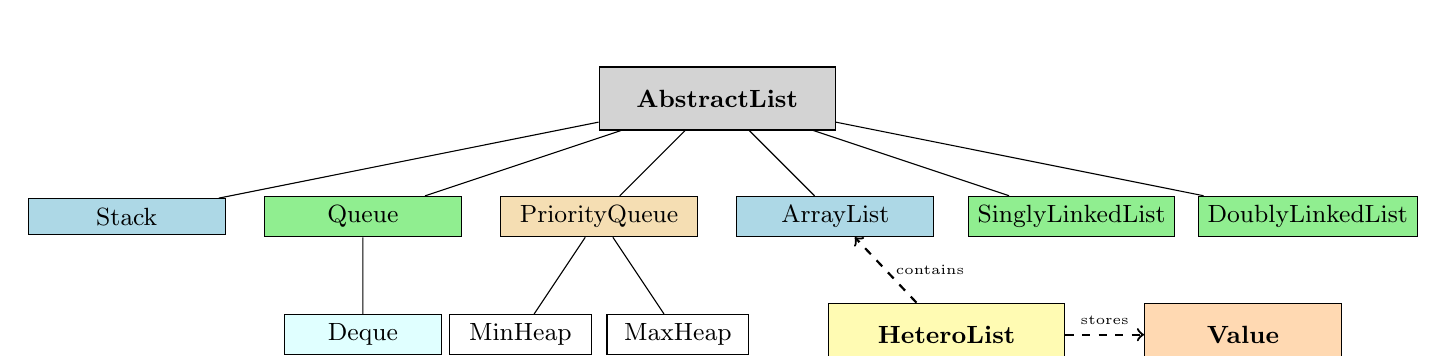
\begin{tikzpicture}[
    node distance=1.5cm,
    every node/.style={font=\small},
    level 1/.style={sibling distance=3cm},
    level 2/.style={sibling distance=2cm}
]

% Root
\node[draw, rectangle, fill=lightgray, minimum width=3cm, minimum height=0.8cm] (abstract) {\textbf{AbstractList}}
    child {node[draw, rectangle, fill=lightblue, minimum width=2.5cm] (stack) {Stack}}
    child {node[draw, rectangle, fill=lightgreen, minimum width=2.5cm] (queue) {Queue}
        child {node[draw, rectangle, fill=lightcyan, minimum width=2cm] (deque) {Deque}}
    }
    child {node[draw, rectangle, fill=wheat, minimum width=2.5cm] (pq) {PriorityQueue}
        child {node[draw, rectangle, minimum width=1.8cm] (minheap) {MinHeap}}
        child {node[draw, rectangle, minimum width=1.8cm] (maxheap) {MaxHeap}}
    }
    child {node[draw, rectangle, fill=lightblue, minimum width=2.5cm] (arraylist) {ArrayList}}
    child {node[draw, rectangle, fill=lightgreen, minimum width=2.5cm] (singly) {SinglyLinkedList}}
    child {node[draw, rectangle, fill=lightgreen, minimum width=2.5cm] (doubly) {DoublyLinkedList}};

% HeteroList separately
\node[draw, rectangle, fill=yellow!30, minimum width=3cm, minimum height=0.8cm, below=3cm of abstract, right=1cm of maxheap] (hetero) {\textbf{HeteroList}};
\draw[->, thick, dashed] (hetero) -- (arraylist) node[midway, right, font=\tiny] {contains};

% Value class
\node[draw, rectangle, fill=orange!30, minimum width=2.5cm, minimum height=0.8cm, right=1cm of hetero] (value) {\textbf{Value}};
\draw[->, thick, dashed] (hetero) -- (value) node[midway, above, font=\tiny] {stores};

\end{tikzpicture}
\caption{Complete Class Hierarchy Overview}
\label{fig:complete-hierarchy}
\end{figure}

\subsection{The Value Class - Type Erasure Foundation}

The biggest challenge was making C++ store heterogeneous data. We created a \texttt{Value} class that can hold any of six types using type erasure:

\begin{center}
\begin{tabular}{|l|l|l|}
\hline
\textbf{Type} & \textbf{C++ Storage} & \textbf{Example} \\
\hline
Null & (flag) & \texttt{Value()} \\
Bool & \texttt{bool} & \texttt{Value(true)} \\
Int & \texttt{long long} & \texttt{Value(42)} \\
Double & \texttt{double} & \texttt{Value(3.14)} \\
String & \texttt{std::string} & \texttt{Value(``hello'')} \\
List & \texttt{shared\_ptr<HeteroList>} & Nested lists \\
\hline
\end{tabular}
\end{center}

\begin{figure}[H]
\centering
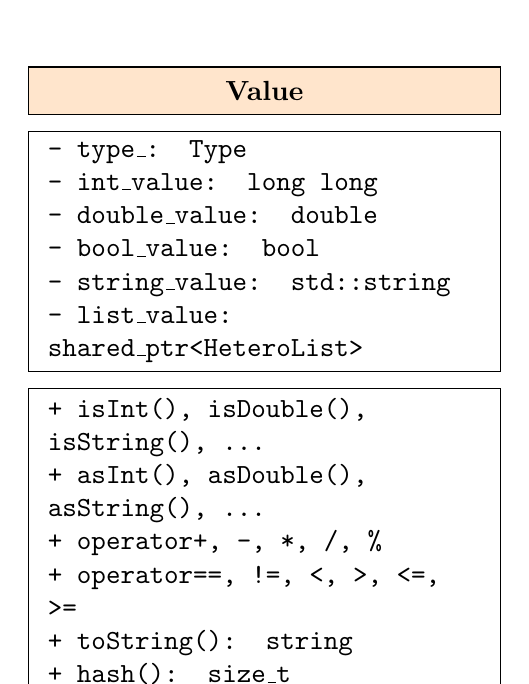
\begin{tikzpicture}[node distance=0.2cm]
\node[draw, rectangle, minimum width=6cm, minimum height=0.6cm, fill=orange!20] (title) {\textbf{Value}};
\node[draw, rectangle, minimum width=6cm, minimum height=2cm, below=of title, anchor=north] (attrs) {
    \begin{minipage}{5.5cm}
    \texttt{- type\_: Type} \\
    \texttt{- int\_value: long long} \\
    \texttt{- double\_value: double} \\
    \texttt{- bool\_value: bool} \\
    \texttt{- string\_value: std::string} \\
    \texttt{- list\_value: shared\_ptr<HeteroList>}
    \end{minipage}
};
\node[draw, rectangle, minimum width=6cm, minimum height=3cm, below=of attrs, anchor=north] (methods) {
    \begin{minipage}{5.5cm}
    \texttt{+ isInt(), isDouble(), isString(), ...} \\
    \texttt{+ asInt(), asDouble(), asString(), ...} \\
    \texttt{+ operator+, -, *, /, \%} \\
    \texttt{+ operator==, !=, <, >, <=, >=} \\
    \texttt{+ toString(): string} \\
    \texttt{+ hash(): size\_t}
    \end{minipage}
};
\end{tikzpicture}
\caption{Value Class Structure with Type Erasure}
\label{fig:value-class}
\end{figure}

\textbf{Design Decision:} We used separate member variables instead of \texttt{std::variant} because:
\begin{itemize}
    \item Simpler to understand and debug
    \item Easier to handle non-trivial types like \texttt{std::string}
    \item More control over comparison and arithmetic operators
\end{itemize}

\textbf{Design Decision:} We used \texttt{shared\_ptr} for nested lists to:
\begin{itemize}
    \item Avoid deep copying when lists are passed around
    \item Enable reference counting for automatic memory management
    \item Allow circular references (though we don't specifically use them)
\end{itemize}

\subsection{AbstractList - Root Abstract Class}

\begin{figure}[H]
\centering
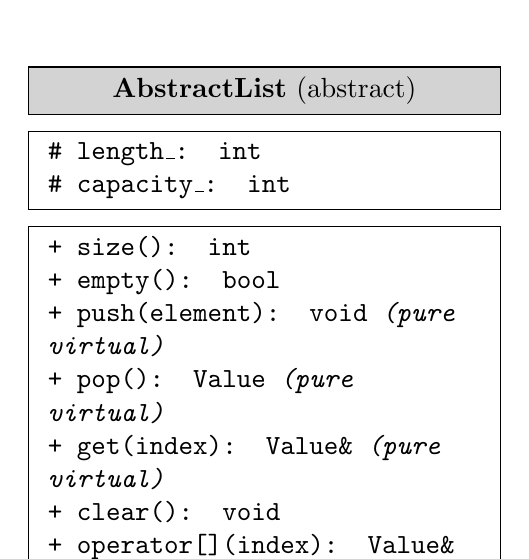
\begin{tikzpicture}[node distance=0.2cm]
\node[draw, rectangle, minimum width=6cm, minimum height=0.6cm, fill=lightgray] (title) {\textbf{AbstractList} (abstract)};
\node[draw, rectangle, minimum width=6cm, minimum height=1cm, below=of title, anchor=north] (attrs) {
    \begin{minipage}{5.5cm}
    \texttt{\# length\_: int} \\
    \texttt{\# capacity\_: int}
    \end{minipage}
};
\node[draw, rectangle, minimum width=6cm, minimum height=2.5cm, below=of attrs, anchor=north] (methods) {
    \begin{minipage}{5.5cm}
    \texttt{+ size(): int} \\
    \texttt{+ empty(): bool} \\
    \texttt{+ push(element): void \textit{(pure virtual)}} \\
    \texttt{+ pop(): Value \textit{(pure virtual)}} \\
    \texttt{+ get(index): Value\& \textit{(pure virtual)}} \\
    \texttt{+ clear(): void} \\
    \texttt{+ operator[](index): Value\&}
    \end{minipage}
};
\end{tikzpicture}
\caption{AbstractList Interface}
\label{fig:abstractlist}
\end{figure}

\textbf{Purpose:} Provides fundamental list operations as an interface contract for all concrete implementations.

\textbf{API Promises:}
\begin{itemize}
    \item \texttt{size()}: Returns current number of elements - O(1)
    \item \texttt{empty()}: Returns true if list has no elements - O(1)
    \item \texttt{push(element)}: Add element (implementation varies by subclass)
    \item \texttt{pop()}: Remove and return an element (implementation varies)
    \item \texttt{clear()}: Remove all elements - O(n)
\end{itemize}

\subsection{Stack Implementation}

\begin{figure}[H]
\centering
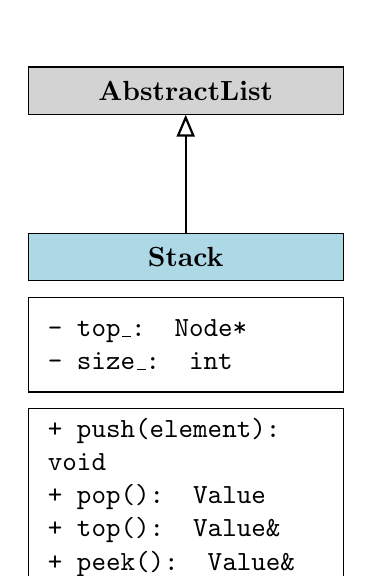
\begin{tikzpicture}[node distance=0.2cm]
% AbstractList
\node[draw, rectangle, minimum width=4cm, minimum height=0.6cm, fill=lightgray] (abstract) {\textbf{AbstractList}};

% Stack
\node[draw, rectangle, minimum width=4cm, minimum height=0.6cm, fill=lightblue, below=1.5cm of abstract] (stack-title) {\textbf{Stack}};
\node[draw, rectangle, minimum width=4cm, minimum height=1.2cm, below=of stack-title, anchor=north] (stack-attrs) {
    \begin{minipage}{3.5cm}
    \texttt{- top\_: Node*} \\
    \texttt{- size\_: int}
    \end{minipage}
};
\node[draw, rectangle, minimum width=4cm, minimum height=2cm, below=of stack-attrs, anchor=north] (stack-methods) {
    \begin{minipage}{3.5cm}
    \texttt{+ push(element): void} \\
    \texttt{+ pop(): Value} \\
    \texttt{+ top(): Value\&} \\
    \texttt{+ peek(): Value\&}
    \end{minipage}
};

\draw[inheritance] (stack-title.north) -- (abstract.south);
\end{tikzpicture}
\caption{Stack Class - LIFO Container}
\label{fig:stack}
\end{figure}

\textbf{Purpose:} Last-In-First-Out (LIFO) data structure with top-only access.

\textbf{Key Design Features:}
\begin{itemize}
    \item \textbf{Single Access Point}: All operations occur at the top
    \item \textbf{Node-Based Storage}: Uses linked nodes for dynamic sizing
    \item \textbf{Top Element Caching}: Maintains pointer to top for O(1) access
    \item \textbf{Exception Safety}: Throws underflow exceptions when popping from empty stack
\end{itemize}

\textbf{API Promises:}
\begin{itemize}
    \item \texttt{push(element)}: Add element to top - O(1)
    \item \texttt{pop()}: Remove and return top element - O(1)
    \item \texttt{top()}: Return top element without removing - O(1)
    \item \texttt{peek()}: Alias for top() - O(1)
\end{itemize}

\subsection{Queue Family}

\begin{figure}[H]
\centering
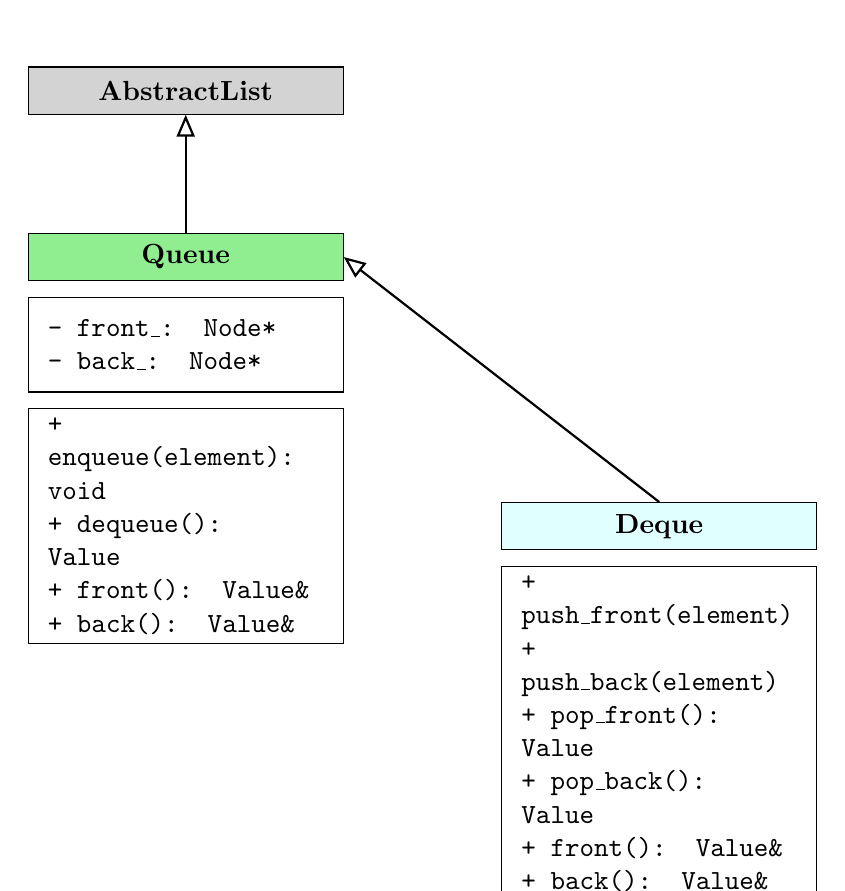
\begin{tikzpicture}[node distance=0.2cm]
% AbstractList
\node[draw, rectangle, minimum width=4cm, minimum height=0.6cm, fill=lightgray] (abstract) {\textbf{AbstractList}};

% Queue
\node[draw, rectangle, minimum width=4cm, minimum height=0.6cm, fill=lightgreen, below=1.5cm of abstract] (queue-title) {\textbf{Queue}};
\node[draw, rectangle, minimum width=4cm, minimum height=1.2cm, below=of queue-title, anchor=north] (queue-attrs) {
    \begin{minipage}{3.5cm}
    \texttt{- front\_: Node*} \\
    \texttt{- back\_: Node*}
    \end{minipage}
};
\node[draw, rectangle, minimum width=4cm, minimum height=2cm, below=of queue-attrs, anchor=north] (queue-methods) {
    \begin{minipage}{3.5cm}
    \texttt{+ enqueue(element): void} \\
    \texttt{+ dequeue(): Value} \\
    \texttt{+ front(): Value\&} \\
    \texttt{+ back(): Value\&}
    \end{minipage}
};

% Deque
\node[draw, rectangle, minimum width=4cm, minimum height=0.6cm, fill=lightcyan, right=2cm of queue-methods] (deque-title) {\textbf{Deque}};
\node[draw, rectangle, minimum width=4cm, minimum height=2.5cm, below=of deque-title, anchor=north] (deque-methods) {
    \begin{minipage}{3.5cm}
    \texttt{+ push\_front(element)} \\
    \texttt{+ push\_back(element)} \\
    \texttt{+ pop\_front(): Value} \\
    \texttt{+ pop\_back(): Value} \\
    \texttt{+ front(): Value\&} \\
    \texttt{+ back(): Value\&}
    \end{minipage}
};

\draw[inheritance] (queue-title.north) -- (abstract.south);
\draw[inheritance] (deque-title.north) -- (queue-title.east);
\end{tikzpicture}
\caption{Queue Family - FIFO and Double-Ended Containers}
\label{fig:queue-family}
\end{figure}

\textbf{Queue Purpose:} First-In-First-Out (FIFO) container with front and back access.

\textbf{Base Queue Features:}
\begin{itemize}
    \item \textbf{Dual-Pointer Design}: Maintains front and back pointers for O(1) operations
    \item \textbf{FIFO Semantics}: Elements added at back, removed from front
    \item \textbf{Flexible Interface}: Supports both push/pop and enqueue/dequeue terminology
\end{itemize}

\textbf{Deque Capabilities:}
\begin{itemize}
    \item \textbf{Double-Ended Operations}: Insertion and removal at both ends
    \item \textbf{Versatile Usage}: Can function as both stack and queue
    \item \textbf{Optimized Storage}: Circular buffer implementation for space efficiency
\end{itemize}

\subsection{PriorityQueue and Heaps}

\begin{figure}[H]
\centering
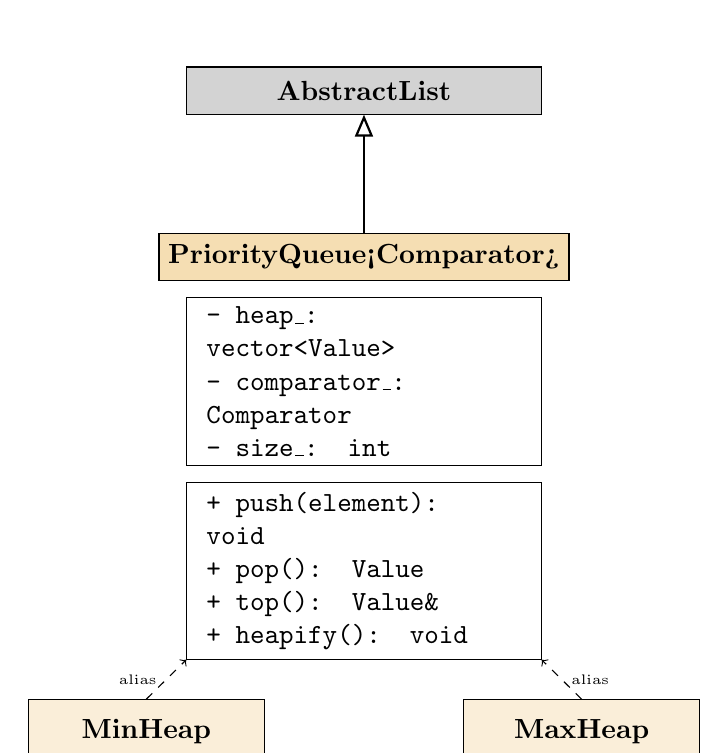
\begin{tikzpicture}[node distance=0.2cm]
% AbstractList
\node[draw, rectangle, minimum width=4.5cm, minimum height=0.6cm, fill=lightgray] (abstract) {\textbf{AbstractList}};

% PriorityQueue
\node[draw, rectangle, minimum width=4.5cm, minimum height=0.6cm, fill=wheat, below=1.5cm of abstract] (pq-title) {\textbf{PriorityQueue<Comparator>}};
\node[draw, rectangle, minimum width=4.5cm, minimum height=1.5cm, below=of pq-title, anchor=north] (pq-attrs) {
    \begin{minipage}{4cm}
    \texttt{- heap\_: vector<Value>} \\
    \texttt{- comparator\_: Comparator} \\
    \texttt{- size\_: int}
    \end{minipage}
};
\node[draw, rectangle, minimum width=4.5cm, minimum height=2cm, below=of pq-attrs, anchor=north] (pq-methods) {
    \begin{minipage}{4cm}
    \texttt{+ push(element): void} \\
    \texttt{+ pop(): Value} \\
    \texttt{+ top(): Value\&} \\
    \texttt{+ heapify(): void}
    \end{minipage}
};

% MinHeap and MaxHeap
\node[draw, rectangle, minimum width=3cm, minimum height=0.8cm, fill=wheat!50, below left=0.5cm and -1cm of pq-methods] (minheap) {\textbf{MinHeap}};
\node[draw, rectangle, minimum width=3cm, minimum height=0.8cm, fill=wheat!50, below right=0.5cm and -1cm of pq-methods] (maxheap) {\textbf{MaxHeap}};

\draw[inheritance] (pq-title.north) -- (abstract.south);
\draw[dashed, ->] (minheap.north) -- (pq-methods.south west) node[midway, left, font=\tiny] {alias};
\draw[dashed, ->] (maxheap.north) -- (pq-methods.south east) node[midway, right, font=\tiny] {alias};
\end{tikzpicture}
\caption{PriorityQueue with Heap Specializations}
\label{fig:priorityqueue}
\end{figure}

\textbf{Purpose:} Queue where elements are served based on priority rather than insertion order.

\textbf{PriorityQueue Features:}
\begin{itemize}
    \item \textbf{Heap-Based Implementation}: Uses binary heap for efficient priority ordering
    \item \textbf{Customizable Comparator}: Allows user-defined priority functions
    \item \textbf{Logarithmic Complexity}: O(log n) insertion and removal
    \item \textbf{Constant Top Access}: O(1) access to highest priority element
\end{itemize}

\textbf{API Promises:}
\begin{itemize}
    \item \texttt{push(element)}: Insert maintaining priority order - O(log n)
    \item \texttt{pop()}: Remove and return highest priority element - O(log n)
    \item \texttt{top()}: Return highest priority element - O(1)
\end{itemize}

\textbf{MinHeap} guarantees smallest element has highest priority.\\
\textbf{MaxHeap} guarantees largest element has highest priority.

\subsection{ArrayList - Dynamic Array}

\begin{figure}[H]
\centering
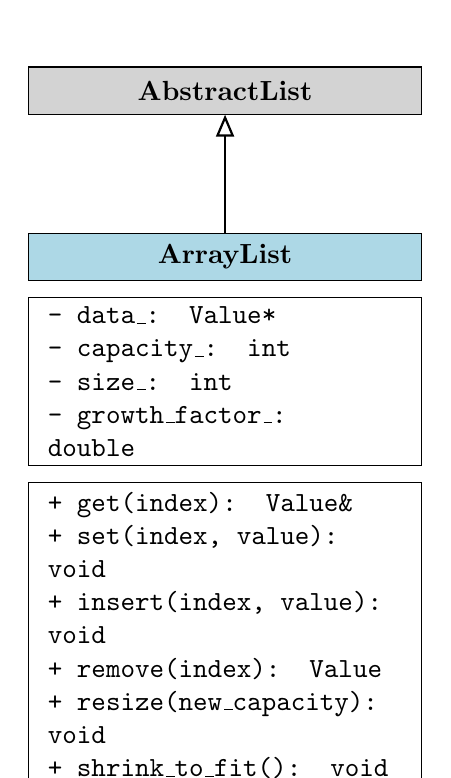
\begin{tikzpicture}[node distance=0.2cm]
% AbstractList
\node[draw, rectangle, minimum width=5cm, minimum height=0.6cm, fill=lightgray] (abstract) {\textbf{AbstractList}};

% ArrayList
\node[draw, rectangle, minimum width=5cm, minimum height=0.6cm, fill=lightblue, below=1.5cm of abstract] (al-title) {\textbf{ArrayList}};
\node[draw, rectangle, minimum width=5cm, minimum height=1.5cm, below=of al-title, anchor=north] (al-attrs) {
    \begin{minipage}{4.5cm}
    \texttt{- data\_: Value*} \\
    \texttt{- capacity\_: int} \\
    \texttt{- size\_: int} \\
    \texttt{- growth\_factor\_: double}
    \end{minipage}
};
\node[draw, rectangle, minimum width=5cm, minimum height=2.5cm, below=of al-attrs, anchor=north] (al-methods) {
    \begin{minipage}{4.5cm}
    \texttt{+ get(index): Value\&} \\
    \texttt{+ set(index, value): void} \\
    \texttt{+ insert(index, value): void} \\
    \texttt{+ remove(index): Value} \\
    \texttt{+ resize(new\_capacity): void} \\
    \texttt{+ shrink\_to\_fit(): void}
    \end{minipage}
};

\draw[inheritance] (al-title.north) -- (abstract.south);
\end{tikzpicture}
\caption{ArrayList - Contiguous Memory Implementation}
\label{fig:arraylist}
\end{figure}

\textbf{Purpose:} Resizable array with random access capabilities and contiguous memory layout.

\textbf{Key Characteristics:}
\begin{itemize}
    \item \textbf{Contiguous Memory}: Array-based storage for cache efficiency
    \item \textbf{Dynamic Resizing}: Automatic capacity expansion with configurable growth factor
    \item \textbf{Random Access}: O(1) indexed access to elements
    \item \textbf{Amortized Performance}: O(1) amortized insertion at end
\end{itemize}

\textbf{API Promises:}
\begin{itemize}
    \item \texttt{get(index)}: Direct array access - O(1)
    \item \texttt{push(element)}: Add to end, resize if needed - Amortized O(1)
    \item \texttt{insert(index, element)}: Insert at position - O(n)
    \item \texttt{remove(index)}: Remove element at index - O(n)
    \item \texttt{resize(new\_capacity)}: Change array capacity - O(n)
    \item \texttt{shrink\_to\_fit()}: Reduce capacity to match size - O(n)
\end{itemize}

\subsection{LinkedList Family}

\begin{figure}[H]
\centering
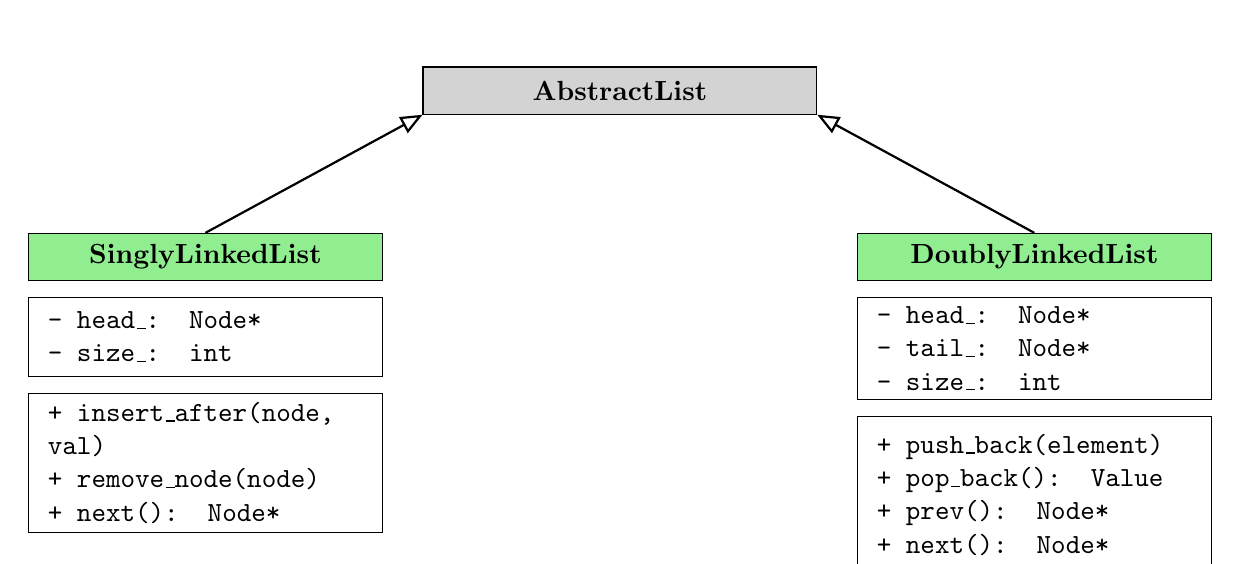
\begin{tikzpicture}[node distance=0.2cm]
% AbstractList
\node[draw, rectangle, minimum width=5cm, minimum height=0.6cm, fill=lightgray] (abstract) {\textbf{AbstractList}};

% SinglyLinkedList
\node[draw, rectangle, minimum width=4.5cm, minimum height=0.6cm, fill=lightgreen, below left=1.5cm and 0.5cm of abstract] (singly-title) {\textbf{SinglyLinkedList}};
\node[draw, rectangle, minimum width=4.5cm, minimum height=1cm, below=of singly-title, anchor=north] (singly-attrs) {
    \begin{minipage}{4cm}
    \texttt{- head\_: Node*} \\
    \texttt{- size\_: int}
    \end{minipage}
};
\node[draw, rectangle, minimum width=4.5cm, minimum height=1.5cm, below=of singly-attrs, anchor=north] (singly-methods) {
    \begin{minipage}{4cm}
    \texttt{+ insert\_after(node, val)} \\
    \texttt{+ remove\_node(node)} \\
    \texttt{+ next(): Node*}
    \end{minipage}
};

% DoublyLinkedList
\node[draw, rectangle, minimum width=4.5cm, minimum height=0.6cm, fill=lightgreen, below right=1.5cm and 0.5cm of abstract] (doubly-title) {\textbf{DoublyLinkedList}};
\node[draw, rectangle, minimum width=4.5cm, minimum height=1.2cm, below=of doubly-title, anchor=north] (doubly-attrs) {
    \begin{minipage}{4cm}
    \texttt{- head\_: Node*} \\
    \texttt{- tail\_: Node*} \\
    \texttt{- size\_: int}
    \end{minipage}
};
\node[draw, rectangle, minimum width=4.5cm, minimum height=2cm, below=of doubly-attrs, anchor=north] (doubly-methods) {
    \begin{minipage}{4cm}
    \texttt{+ push\_back(element)} \\
    \texttt{+ pop\_back(): Value} \\
    \texttt{+ prev(): Node*} \\
    \texttt{+ next(): Node*}
    \end{minipage}
};

\draw[inheritance] (singly-title.north) -- (abstract.south west);
\draw[inheritance] (doubly-title.north) -- (abstract.south east);
\end{tikzpicture}
\caption{LinkedList Family - Node-Based Storage}
\label{fig:linkedlist-family}
\end{figure}

\textbf{SinglyLinkedList Features:}
\begin{itemize}
    \item \textbf{Memory Efficient}: Minimal overhead per node (one pointer)
    \item \textbf{Forward Traversal}: Unidirectional iteration capability
    \item \textbf{Dynamic Size}: No pre-allocation required
    \item \textbf{Efficient Head Operations}: O(1) insertion/deletion at beginning
\end{itemize}

\textbf{DoublyLinkedList Features:}
\begin{itemize}
    \item \textbf{Bidirectional Traversal}: Forward and backward iteration
    \item \textbf{Tail Pointer Optimization}: O(1) operations at both ends
    \item \textbf{Flexible Navigation}: Previous/next navigation in constant time
    \item \textbf{Enhanced Iterator}: Support for reverse iteration patterns
\end{itemize}

\subsection{HeteroList - Functional-OO Wrapper}

\begin{figure}[H]
\centering
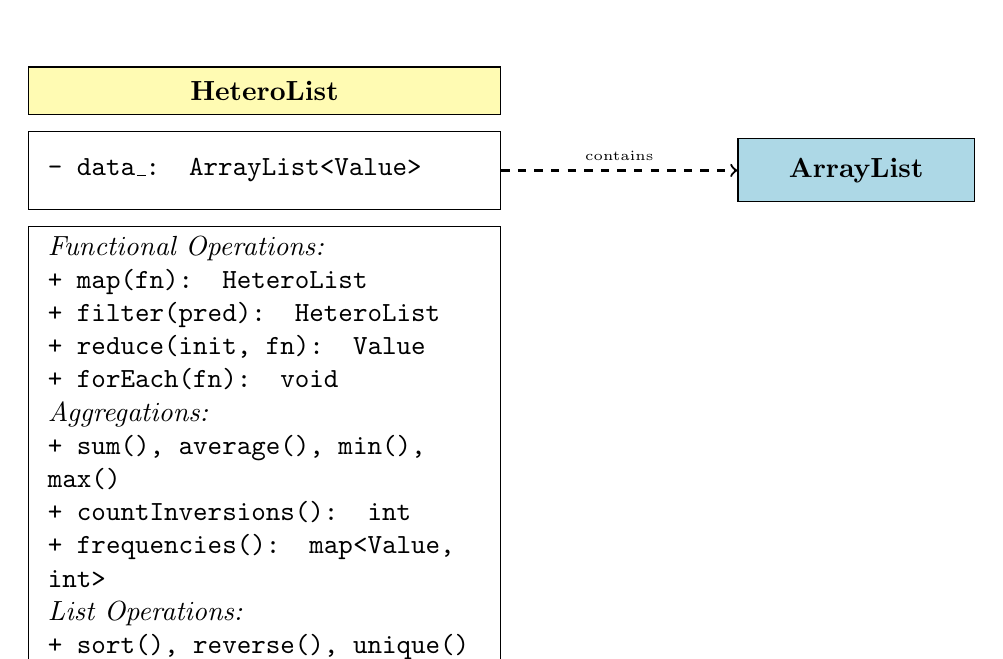
\begin{tikzpicture}[node distance=0.2cm]
% HeteroList
\node[draw, rectangle, minimum width=6cm, minimum height=0.6cm, fill=yellow!30] (hetero-title) {\textbf{HeteroList}};
\node[draw, rectangle, minimum width=6cm, minimum height=1cm, below=of hetero-title, anchor=north] (hetero-attrs) {
    \begin{minipage}{5.5cm}
    \texttt{- data\_: ArrayList<Value>}
    \end{minipage}
};
\node[draw, rectangle, minimum width=6cm, minimum height=4cm, below=of hetero-attrs, anchor=north] (hetero-methods) {
    \begin{minipage}{5.5cm}
    \textit{Functional Operations:} \\
    \texttt{+ map(fn): HeteroList} \\
    \texttt{+ filter(pred): HeteroList} \\
    \texttt{+ reduce(init, fn): Value} \\
    \texttt{+ forEach(fn): void} \\
    \textit{Aggregations:} \\
    \texttt{+ sum(), average(), min(), max()} \\
    \texttt{+ countInversions(): int} \\
    \texttt{+ frequencies(): map<Value, int>} \\
    \textit{List Operations:} \\
    \texttt{+ sort(), reverse(), unique()}
    \end{minipage}
};

% ArrayList connection
\node[draw, rectangle, minimum width=3cm, minimum height=0.8cm, fill=lightblue, right=3cm of hetero-attrs] (arraylist) {\textbf{ArrayList}};
\draw[->, thick, dashed] (hetero-attrs.east) -- (arraylist.west) node[midway, above, font=\tiny] {contains};

\end{tikzpicture}
\caption{HeteroList - Contain-and-Delegate Design}
\label{fig:heterolist}
\end{figure}

\textbf{Purpose:} User-facing specification that adds functional programming operations on top of ArrayList storage.

\textbf{Design Philosophy:}
\begin{itemize}
    \item \textbf{Contain-and-Delegate}: Wraps ArrayList rather than inheriting
    \item \textbf{Specification vs Implementation}: Users see functional interface, not storage details
    \item \textbf{Composable Operations}: Methods can be chained for expressive code
    \item \textbf{Type Safety}: Value class ensures runtime type checking
\end{itemize}

\textbf{Why Contain-and-Delegate?}
\begin{itemize}
    \item Can swap ArrayList for another implementation without breaking user code
    \item Hides capacity management and resizing from users
    \item Adds domain-specific operations without modifying base class
    \item Follows composition-over-inheritance principle
\end{itemize}

\subsection{Performance Comparison}

\begin{table}[H]
\centering
\begin{tabular}{|l|c|c|c|c|}
\hline
\textbf{Operation} & \textbf{ArrayList} & \textbf{SinglyLinked} & \textbf{DoublyLinked} & \textbf{Stack/Queue} \\
\hline
Access by Index & O(1) & O(n) & O(n) & N/A \\
Insert at Head & O(n) & O(1) & O(1) & O(1) \\
Insert at Tail & O(1)* & O(n) & O(1) & O(1) \\
Insert at Middle & O(n) & O(1)** & O(1)** & N/A \\
Delete at Head & O(n) & O(1) & O(1) & O(1) \\
Delete at Tail & O(1) & O(n) & O(1) & O(1) \\
Search & O(n) & O(n) & O(n) & O(n) \\
Memory per Element & Low & Medium & High & Medium \\
Cache Performance & Excellent & Poor & Poor & Medium \\
\hline
\end{tabular}
\caption{Performance Characteristics (* Amortized, ** At known position)}
\label{tab:performance}
\end{table}

\section{Library Implementation}

\subsection{Value Class API}

\begin{center}
\begin{tabular}{|l|p{9cm}|}
\hline
\textbf{Method} & \textbf{Description} \\
\hline
\texttt{type()} & Returns the Type enum \\
\texttt{isNull()}, \texttt{isBool()}, \texttt{isInt()}, \texttt{isDouble()}, \texttt{isString()}, \texttt{isList()} & Type predicates \\
\texttt{isNumeric()} & True if Int or Double \\
\texttt{asInt()}, \texttt{asDouble()}, \texttt{asBool()}, \texttt{asString()}, \texttt{asList()} & Type conversion (throws on mismatch) \\
\texttt{toString()} & String representation \\
\texttt{==}, \texttt{!=}, \texttt{<}, \texttt{>}, \texttt{<=}, \texttt{>=} & Comparison operators \\
\texttt{+}, \texttt{-}, \texttt{*}, \texttt{/}, \texttt{\%} & Arithmetic operators \\
\texttt{hash()} & For use in hash maps \\
\hline
\end{tabular}
\end{center}

\subsection{HeteroList Basic Operations}

\begin{center}
\begin{tabular}{|l|p{9cm}|}
\hline
\textbf{Method} & \textbf{Description} \\
\hline
\texttt{size()} & Number of elements \\
\texttt{empty()} & Check if empty \\
\texttt{push(value)} & Append element \\
\texttt{pop()} & Remove and return last \\
\texttt{get(index)} / \texttt{operator[]} & Access by index \\
\texttt{set(index, value)} & Update element \\
\texttt{insert(index, value)} & Insert at position \\
\texttt{remove(index)} & Remove from position \\
\texttt{indexOf(value)} & Find element (-1 if not found) \\
\texttt{contains(value)} & Check existence \\
\texttt{sort()} / \texttt{sortDescending()} & Sort in place \\
\texttt{reverse()} & Reverse in place \\
\hline
\end{tabular}
\end{center}

\subsection{Functional Operations}

\begin{center}
\begin{tabular}{|l|p{10cm}|}
\hline
\textbf{Method} & \textbf{Description} \\
\hline
\texttt{map} & Transform each element \\
\texttt{filter} & Keep matching elements \\
\texttt{reduce} & Combine into single value \\
\texttt{forEach} & Execute for each element \\
\texttt{any} & True if any match \\
\texttt{all} & True if all match \\
\texttt{count} & Count matches \\
\texttt{find} & Find first match \\
\texttt{take} & First n elements \\
\texttt{drop} & Skip first n elements \\
\texttt{partition} & Split by predicate \\
\texttt{unique} & Remove duplicates \\
\texttt{flatten} & Flatten nested lists \\
\hline
\end{tabular}
\end{center}

\subsection{Aggregation Operations}

\begin{center}
\begin{tabular}{|l|p{9cm}|}
\hline
\textbf{Method} & \textbf{Description} \\
\hline
\texttt{sum()} & Sum of numeric elements \\
\texttt{product()} & Product of numeric elements \\
\texttt{average()} & Mean of numeric elements \\
\texttt{min()} / \texttt{max()} & Extreme values \\
\texttt{countInversions()} & Count out-of-order pairs \\
\texttt{frequencies()} & Count each unique element \\
\hline
\end{tabular}
\end{center}

\subsection{Performance Characteristics}

\begin{center}
\begin{tabular}{|l|c|c|c|}
\hline
\textbf{Operation} & \textbf{ArrayList} & \textbf{SinglyLinkedList} & \textbf{DoublyLinkedList} \\
\hline
\texttt{push} (end) & O(1)* & O(1) & O(1) \\
\texttt{pop} (end) & O(1) & O(n) & O(1) \\
\texttt{get(index)} & O(1) & O(n) & O(n/2) \\
\texttt{insert(0)} & O(n) & O(1) & O(1) \\
\texttt{search} & O(n) & O(n) & O(n) \\
\texttt{sort} & O(n log n) & N/A & N/A \\
\hline
\end{tabular}
\end{center}

* Amortized, with occasional O(n) for reallocation

\section{Use Case 1: Keyword Frequency Counter}

\subsection{Overview}

This use case demonstrates a \textbf{pure functional programming approach} to counting keyword occurrences in text files. Instead of using traditional loops and hash maps, we use \texttt{map()}, \texttt{count()}, \texttt{forEach()}, and \texttt{sort()}.

\subsection{How It Uses the Library}

\begin{lstlisting}[language=C++]
// Step 1: Read keywords into HeteroList
HeteroList keywords = readKeywords(keywordFile);

// Step 2: Read ALL words from all files into one HeteroList
HeteroList allWords;
files.forEach([&](const Value& filePath) {
    HeteroList fileWords = readWordsFromFile(filePath.asString());
    // Add all words to allWords
});

// Step 3: Transform keywords to [keyword, count] pairs
HeteroList results = keywords.map([&allWords](const Value& keyword) {
    int freq = allWords.count([&](const Value& word) {
        return matches(word, keyword);
    });
    return Value(makeList({keyword, Value(freq)}));
});

// Step 4: Sort by count descending
results.sort(/* comparator */);

// Step 5: Output using forEach
results.forEach([](const Value& pair) {
    // Print each [keyword, count] pair
});
\end{lstlisting}

\subsection{Functional-OO Concepts Demonstrated}

\begin{center}
\begin{tabular}{|l|p{9cm}|}
\hline
\textbf{Concept} & \textbf{How It's Used} \\
\hline
Higher-Order Functions & \texttt{map()}, \texttt{forEach()}, \texttt{count()} take lambda functions \\
Transformation & \texttt{map()} transforms keywords to [keyword, count] pairs \\
Aggregation & \texttt{count()} with predicate replaces manual counting loops \\
Custom Sorting & \texttt{sort()} with comparator for descending order \\
Nested Lists & Results stored as [[kw1, count1], [kw2, count2], ...] \\
\hline
\end{tabular}
\end{center}

\section{Use Case 2: Network Stream Processor}

\subsection{Overview}

A client-server application demonstrating \textbf{real-time streaming} of heterogeneous data over TCP/IP sockets. The server generates random data of mixed types, and the client receives, categorizes, sorts, and displays live statistics.

\subsection{How It Uses the Library}

\begin{lstlisting}[language=C++]
// Client maintains three lists by type
HeteroList integers_, doubles_, strings_;

// Parse incoming data
Value parseValue(const std::string& line) {
    auto [type, valueStr] = split(line, ':');
    if (type == "INT") return Value(std::stoll(valueStr));
    // ...
    return Value();
}

// Categorize by type
if (val.isInt()) integers_.push(val);
else if (val.isDouble()) doubles_.push(val);
else if (val.isString()) strings_.push(val);

// Real-time aggregations
integers_.sum();
integers_.average();
integers_.min();
integers_.max();
integers_.countInversions();
strings_.frequencies();
\end{lstlisting}

\subsection{Features Demonstrated}

\begin{center}
\begin{tabular}{|l|p{8cm}|}
\hline
\textbf{Feature} & \textbf{Library Methods Used} \\
\hline
Type Checking & \texttt{isInt()}, \texttt{isDouble()}, \texttt{isString()} \\
Real-Time Sorting & \texttt{sort()} called on each update \\
Aggregations & \texttt{sum()}, \texttt{average()}, \texttt{min()}, \texttt{max()} \\
Disorder Metric & \texttt{countInversions()} \\
Frequency Analysis & \texttt{frequencies()} \\
Heterogeneous Storage & All types in \texttt{HeteroList} \\
\hline
\end{tabular}
\end{center}

\section{Use Case 3: CLI Application}

\subsection{Overview}

A command-line interface that wraps the HeteroList library with \textbf{JSON-based input/output}. This allows external programs (like Python scripts) to use our C++ implementation through subprocess calls.

\subsection{Design Rationale}

We wanted to demonstrate that our library could be used from other languages. The CLI accepts JSON arrays as input and returns JSON results, making it easy to integrate with Python, Node.js, or shell scripts.

\subsection{Commands Supported}

\begin{center}
\begin{tabular}{|l|p{10cm}|}
\hline
\textbf{Command} & \textbf{Example} \\
\hline
\texttt{create} & \texttt{./hetero\_cli create "[1, 2, \textbackslash"hello\textbackslash"]"} \\
\texttt{sort} & \texttt{./hetero\_cli sort "[5, 3, 8]" asc} \\
\texttt{filter} & \texttt{./hetero\_cli filter "[1, \textbackslash"hi\textbackslash", 2]" int} \\
\texttt{map} & \texttt{./hetero\_cli map "[1, 2, 3]" square} \\
\texttt{reduce} & \texttt{./hetero\_cli reduce "[10, 20]" sum} \\
\texttt{stats} & \texttt{./hetero\_cli stats "[1, 2, 3]"} \\
\texttt{partition} & \texttt{./hetero\_cli partition "[1, 2, 3]" even} \\
\hline
\end{tabular}
\end{center}

\subsection{Map Operations}

\begin{center}
\begin{tabular}{|l|l|}
\hline
\textbf{Operation} & \textbf{Effect} \\
\hline
\texttt{double} & Multiply numeric values by 2 \\
\texttt{square} & Square numeric values \\
\texttt{negate} & Negate numeric values \\
\texttt{increment} & Add 1 \\
\texttt{decrement} & Subtract 1 \\
\texttt{uppercase} & Convert strings to uppercase \\
\texttt{lowercase} & Convert strings to lowercase \\
\hline
\end{tabular}
\end{center}

\subsection{Filter Types}

\begin{center}
\begin{tabular}{|l|l|}
\hline
\textbf{Type} & \textbf{Matches} \\
\hline
\texttt{int} & Integer values only \\
\texttt{double} & Floating-point values only \\
\texttt{string} & String values only \\
\texttt{bool} & Boolean values only \\
\texttt{numeric} & Int + Double \\
\texttt{even} / \texttt{odd} & Even/odd integers \\
\texttt{positive} / \texttt{negative} & Sign-based filtering \\
\hline
\end{tabular}
\end{center}

\subsection{Graceful Error Handling}

For operations requiring numeric values on heterogeneous lists, the CLI filters to numeric values first and includes metadata:

\begin{verbatim}
./hetero_cli stats "[1, \"hello\", 2, true, 3]"
# Output: {"sum": 6, "average": 2, "min": 1, "max": 3, 
#          "count": 3, "total_elements": 5}
\end{verbatim}

\section{Use Case 4: Web Application}

\subsection{Overview}

A Flask-based web interface with Bootstrap 5 dark theme that provides an \textbf{interactive UI} for all HeteroList operations. This is the showcase use case that ties everything together.

\subsection{Architecture}

\begin{verbatim}
+-----------------------------------------------------------+
|             Web Browser (UI)                              |
|          Bootstrap 5 + JavaScript                         |
+-------------------+---------------------------------------+
                    | HTTP/JSON
                    v
+-----------------------------------------------------------+
|            Flask Server (app.py)                          |
|            REST API Endpoints                             |
+-------------------+---------------------------------------+
                    | subprocess
                    v
+-----------------------------------------------------------+
|     C++ CLI (../CLIApp/hetero_cli)                        |
|     Uses HeteroList Implementation Library                |
+-----------------------------------------------------------+
\end{verbatim}

\textbf{Key Design Decision:} We deliberately did NOT reimplement the library in Python. Instead, the Flask server calls the compiled C++ CLI via subprocess. This demonstrates:
\begin{enumerate}
    \item Cross-language interoperability
    \item Reuse of the same implementation
    \item The CLI as an integration layer
\end{enumerate}

\subsection{API Endpoints}

\begin{center}
\small
\begin{longtable}{|l|l|p{6cm}|}
\hline
\textbf{Endpoint} & \textbf{Parameters} & \textbf{Description} \\
\hline
\texttt{/api/create} & \texttt{list} & Validate a list \\
\texttt{/api/sort} & \texttt{list}, \texttt{order} & Sort asc/desc \\
\texttt{/api/filter} & \texttt{list}, \texttt{type} & Filter by predicate \\
\texttt{/api/map} & \texttt{list}, \texttt{operation} & Apply transformation \\
\texttt{/api/reduce} & \texttt{list}, \texttt{operation} & Reduce to single value \\
\texttt{/api/stats} & \texttt{list} & Get statistics \\
\texttt{/api/unique} & \texttt{list} & Remove duplicates \\
\texttt{/api/reverse} & \texttt{list} & Reverse order \\
\texttt{/api/take} & \texttt{list}, \texttt{n} & Take first n \\
\texttt{/api/drop} & \texttt{list}, \texttt{n} & Drop first n \\
\texttt{/api/count} & \texttt{list} & Count by type \\
\texttt{/api/inversions} & \texttt{list} & Count inversions \\
\texttt{/api/frequencies} & \texttt{list} & Element frequencies \\
\texttt{/api/partition} & \texttt{list}, \texttt{type} & Split by predicate \\
\texttt{/api/push} & \texttt{list}, \texttt{value} & Add element \\
\texttt{/api/pop} & \texttt{list} & Remove last \\
\hline
\end{longtable}
\end{center}

\subsection{UI Features}

\begin{itemize}
    \item \textbf{Dark Theme}: Modern gradient-based styling
    \item \textbf{Type Badges}: Color-coded badges (int=blue, double=purple, string=green, bool=red)
    \item \textbf{Quick Add}: Buttons to add random values
    \item \textbf{Sample Data}: Pre-loaded datasets
    \item \textbf{Apply Results}: Use operation result as new input
    \item \textbf{History}: Track and restore previous operations
    \item \textbf{Statistics Cards}: Visual display of sum, average, min, max
    \item \textbf{Frequency Bars}: Visual bar chart for frequencies
\end{itemize}

\subsection{Cross-Platform Support}

On Windows, the Flask server detects the OS and uses WSL to run the Linux-compiled CLI:

\begin{lstlisting}[language=Python]
def get_wsl_path(windows_path):
    # Convert D:\path\to\file to /mnt/d/path/to/file
    ...

if platform.system() == 'Windows':
    cmd = ['wsl'] + cmd  # Prepend wsl
\end{lstlisting}

\section{Testing Strategy}

\subsection{Unit Tests}

We created a comprehensive test file (\texttt{Tests/test\_implementation.cpp}) with 20 test cases covering:

\begin{center}
\begin{tabular}{|l|p{9cm}|}
\hline
\textbf{Test Category} & \textbf{What's Tested} \\
\hline
Basic Operations & push, pop, insert, remove, get, set \\
Functional Operations & map, filter, reduce, forEach \\
Aggregations & sum, average, min, max \\
Sorting & sort, sortDescending, countInversions \\
Type Handling & int, double, string, bool, null, nested lists \\
Edge Cases & empty lists, single elements, type mismatches \\
\hline
\end{tabular}
\end{center}

\subsection{Running Tests}

\begin{verbatim}
make test
\end{verbatim}

All 20 tests pass:

\begin{verbatim}
Running Tests...

Test 1: Basic Push and Pop... PASSED
Test 2: Insert and Remove... PASSED
Test 3: Get and Set... PASSED
...
Test 20: Nested Lists... PASSED

=== All 20 tests passed! ===
\end{verbatim}

\subsection{Incremental Testing}

We tested each component as it was built:
\begin{enumerate}
    \item \textbf{Value class}: Created standalone test for type conversion and operators
    \item \textbf{ArrayList}: Tested push/pop/insert/remove before building HeteroList
    \item \textbf{HeteroList}: Tested functional methods one by one
    \item \textbf{CLI}: Tested each command manually with various inputs
    \item \textbf{Web App}: Tested each API endpoint via browser and curl
\end{enumerate}

\section{Packaging and Build System}

\subsection{Makefile Targets}

We created a single Makefile that builds and runs all components:

\begin{center}
\begin{tabular}{|l|p{9cm}|}
\hline
\textbf{Target} & \textbf{Description} \\
\hline
\texttt{make} & Build and run UC4 (Web App) - \textbf{default} \\
\texttt{make uc1} & Build and run Keyword Frequency Counter \\
\texttt{make uc2} & Build and run Network Stream (server + client) \\
\texttt{make uc3} & Build CLI App and show usage \\
\texttt{make uc4} & Build CLI and run Flask Web App \\
\texttt{make all} & Build all use cases \\
\texttt{make test} & Build and run unit tests \\
\texttt{make clean} & Remove all executables \\
\texttt{make help} & Show all targets \\
\hline
\end{tabular}
\end{center}

\subsection{Automatic Dependency Installation}

The Makefile automatically installs Flask if not present:

\begin{verbatim}
uc4: $(CLI_EXE)
    @python3 -c "import flask" 2>/dev/null || pip3 install flask
    cd $(WEB_DIR) && python3 app.py
\end{verbatim}

\subsection{Single Command Execution}

As required by the assignment, a single command runs the entire application:

\begin{verbatim}
# Default: Run the Web Application
make

# Or specifically:
make uc4
\end{verbatim}

This will:
\begin{enumerate}
    \item Compile the C++ CLI if needed
    \item Install Flask if not present
    \item Start the Flask server
    \item Open the browser to http://127.0.0.1:5000
\end{enumerate}

\subsection{Project Structure}

\begin{verbatim}
Final_Assignment/
+-- Implementation/          # Core library (header-only)
|   +-- myList.hpp          # Main include file
|   +-- Value.hpp           # Type-erased value wrapper
|   +-- HeteroList.hpp      # Main interface
|   +-- AbstractList.hpp    # Abstract base class
|   +-- ArrayList.hpp       # Dynamic array
|   +-- Stack.hpp, Queue.hpp, Deque.hpp
|   +-- PriorityQueue.hpp
|   +-- SinglyLinkedList.hpp, DoublyLinkedList.hpp
|   +-- README.md
|
+-- Tests/
|   +-- test_implementation.cpp
|
+-- UseCases/
|   +-- KeywordFrequency/   # UC1
|   +-- NetworkStream/      # UC2
|   +-- CLIApp/             # UC3
|   +-- WebApp/             # UC4
|   +-- README.md
|
+-- Makefile                # Build system
+-- README.md               # Quick start guide
+-- Report.md               # This file
\end{verbatim}

\section{LLM Assistance Documentation}

We used Claude (Anthropic's AI assistant) throughout the development process. Here we document the prompts used, responses received, and how we incorporated the insights.

\subsection{Initial Library Design}

\textbf{Our Prompt:}

\textit{``We need to extend our heterogeneous list library to support functional operations. We already have the contain-and-delegate design from earlier. Help us implement the Value class for type erasure.''}

\textbf{Claude's Response (summarized):}

Claude suggested a Value class with a Type enum, separate member variables for each type, and provided implementations for constructors, type predicates, and conversion methods.

\textbf{Our Interpretation:}

We agreed with this approach because it cleanly separates specification from implementation. We asked for more details on handling cross-type comparisons.

\textbf{Incorporation:}

Claude helped implement the \texttt{Value} class with its type enum, constructors, and operators. We reviewed the code and made some adjustments to the comparison operators to handle Int vs Double comparisons properly.

\subsection{Functional Operations}

\textbf{Our Prompt:}

\textit{``Add functional programming methods like map, filter, and reduce to the HeteroList class. These should work with lambda functions.''}

\textbf{Claude's Response:}

Claude provided implementations using \texttt{std::function} to accept lambdas. The \texttt{map} function creates a new list with transformed elements, \texttt{filter} keeps elements matching a predicate, and \texttt{reduce} combines elements into a single value.

\textbf{Our Interpretation:}

The implementations looked correct. We tested them with simple examples to verify behavior.

\textbf{Incorporation:}

We added these methods to \texttt{HeteroList.hpp}. Later, we asked Claude to add more methods like \texttt{any}, \texttt{all}, \texttt{count}, \texttt{find}, \texttt{take}, \texttt{drop}, etc.

\subsection{Use Case 1: Keyword Frequency}

\textbf{Our Prompt:}

\textit{``Create a keyword frequency counter that demonstrates the functional programming approach. Instead of using hash maps and loops, use our library's map, count, and forEach methods.''}

\textbf{Claude's Response:}

Claude created \texttt{KeywordFrequency.cpp} that reads keywords into a HeteroList, reads all words from files into another HeteroList, then uses \texttt{map()} with \texttt{count()} to transform keywords into [keyword, count] pairs.

\textbf{Our Suggestion:}

\textit{``Can you also add a summary section that shows total files processed, most frequent keyword, etc.?''}

Claude added the summary output with statistics.

\textbf{Incorporation:}

This became our UC1, demonstrating that functional operations can replace traditional imperative patterns.

\subsection{Use Case 2: Network Stream}

\textbf{Our Prompt:}

\textit{``Create a client-server application that streams heterogeneous data over sockets. The server should generate random ints, doubles, and strings. The client should receive them, store in HeteroList, and show real-time sorted data and statistics.''}

\textbf{Claude's Response:}

Claude created \texttt{Server.cpp} and \texttt{Client.cpp} with TCP socket communication. The client maintains separate lists by type and displays live statistics using our library's aggregation methods.

\textbf{Incorporation:}

We tested this locally and it worked well. The real-time display shows sorted data and statistics updating as new data arrives.

\subsection{Use Case 3 \& 4: CLI and Web App}

\textbf{Our Prompt:}

\textit{``Make a menu-driven app which uses our library to perform functions on heterogeneous lists. Don't create a library in Python - use the underlying C++ compiled versions. Make it locally hosted and basically create APIs which use our C++ implementation.''}

\textbf{Claude's Response:}

Claude suggested creating a CLI wrapper (\texttt{hetero\_cli.cpp}) that accepts JSON input and returns JSON output, then a Flask server that calls this CLI via subprocess. The web UI would be built with Bootstrap.

\textbf{Our Suggestion:}

\textit{``When I click Stats or Inversions on a heterogeneous list, it gives errors. Make it more graceful - filter to numeric values first.''}

Claude modified the CLI to handle heterogeneous lists gracefully by filtering to numeric values before operations like stats and inversions, and including metadata about how many values were used.

\textbf{Incorporation:}

The CLI and Web App became UC3 and UC4. The architecture demonstrates cross-language interoperability while reusing the same C++ implementation.

\subsection{Makefile and Packaging}

\textbf{Our Prompt:}

\textit{``Create a Makefile for Linux which can run all the use cases depending on which one they make. By default run UC4 (web app).''}

\textbf{Claude's Response:}

Claude created a Makefile with targets for each use case, plus \texttt{all}, \texttt{test}, \texttt{clean}, and \texttt{help}.

\textbf{Our Suggestion:}

\textit{``I changed uc2 slightly so that both server and client run. Is there a better way to do this? Also, web app requires flask, so can you install it using pip if it doesn't exist?''}

Claude improved the UC2 target to use backgrounding with sleep, and added Flask auto-install to UC4.

\textbf{Incorporation:}

The final Makefile handles everything with a single \texttt{make} command.

\subsection{Summary of LLM Usage}

\begin{center}
\small
\begin{longtable}{|l|p{5cm}|p{5cm}|}
\hline
\textbf{Task} & \textbf{Our Role} & \textbf{Claude's Role} \\
\hline
Architecture Design & Defined requirements, chose patterns & Suggested implementations \\
Value Class & Reviewed and tested & Implemented type erasure \\
Functional Methods & Specified which methods to add & Implemented map, filter, reduce, etc. \\
Use Cases & Defined what each should demonstrate & Implemented the code \\
Error Handling & Identified edge cases & Added graceful handling \\
Documentation & Specified structure and content & Wrote detailed READMEs \\
Testing & Ran tests, reported issues & Fixed bugs, added test cases \\
Packaging & Specified requirements & Created Makefile \\
\hline
\end{longtable}
\end{center}

\textbf{Key Insight:}

Using an LLM significantly accelerated development, especially for boilerplate code and documentation. However, we still needed to:
\begin{itemize}
    \item Define clear requirements and architecture
    \item Review all generated code
    \item Test thoroughly
    \item Suggest improvements and edge cases
    \item Make design decisions
\end{itemize}

The LLM was most helpful for implementing well-defined tasks and creating documentation, but the design decisions and problem interpretation remained our responsibility.

\section{Conclusion}

\subsection{What We Built}

We created a comprehensive heterogeneous list library in C++ that demonstrates:
\begin{enumerate}
    \item \textbf{Data Abstraction}: The \texttt{Value} class hides type details, the \texttt{HeteroList} class hides storage details
    \item \textbf{Data Independence}: Users interact with \texttt{HeteroList} without knowing about \texttt{ArrayList} internals
    \item \textbf{Functional-OO Integration}: Higher-order functions (\texttt{map}, \texttt{filter}, \texttt{reduce}) with object-oriented structure
    \item \textbf{Practical Applications}: Four use cases showing real-world applicability
\end{enumerate}

\subsection{Design Philosophy Validation}

Our contain-and-delegate approach proved effective:
\begin{itemize}
    \item Clean separation between specification (HeteroList) and implementation (ArrayList)
    \item Easy to add new functional methods without changing storage
    \item Could swap ArrayList for LinkedList without affecting user code
\end{itemize}

\subsection{Lessons Learned}

\begin{enumerate}
    \item \textbf{Type Erasure is Powerful}: The \texttt{Value} class enables Python-like flexibility in C++
    \item \textbf{Functional Operations are Composable}: Chaining \texttt{filter().map().reduce()} is elegant
    \item \textbf{Cross-Language Integration Works}: JSON CLI enables use from Python without reimplementation
    \item \textbf{Testing Early Helps}: Catching issues at the unit test level saved debugging time later
\end{enumerate}

\subsection{Final Deliverable}

A single command runs the complete application:

\begin{verbatim}
make
\end{verbatim}

This compiles everything, installs dependencies, and launches the web interface at http://127.0.0.1:5000, providing interactive access to all library features.

\vspace{1cm}
\begin{center}
\rule{0.5\textwidth}{0.4pt}

\textit{Report prepared for CS F301 - Programming Languages, November 2025}
\end{center}

\end{document}
